\chapter{Conditional Probability and Independence}\label{ch:g12:condprob}

Probability quantifies uncertainty; conditional probability quantifies how
information changes it. Learning that an event $B$ occurred reshapes the
probabilities of all other events --- a mechanism formalized by Bayes and
misused daily in courtrooms and newspapers. This chapter sets up the rules
of conditioning and the exact meaning of independence.

\section{Probability spaces (reminder)}

An experiment with finitely many outcomes is modeled by a \emph{sample
space} $\Omega$ (the set of outcomes) and a probability $\P$ assigning to
each event $A \subseteq \Omega$ a number $\P(A) \in \intcc{0}{1}$, additive
over disjoint unions and with $\P(\Omega) = 1$. Recall the basic rules:
\[
\P(\bar A) = 1 - \P(A),
\qquad
\P(A \cup B) = \P(A) + \P(B) - \P(A \cap B).
\]
When all outcomes are equally likely,
$\P(A) = \frac{\abs A}{\abs\Omega}$ --- and computing probabilities reduces
to the counting techniques of \cref{ch:g12:comb}.

\section{Conditional probability}

\begin{definition}[Conditional probability]\label{def:g12:condprob:cond}
Let $B$ be an event with $\P(B) > 0$. The \emph{probability of $A$ given
$B$}\index{conditional probability} is
\[
\pcond{B}{A} = \frac{\P(A \cap B)}{\P(B)} .
\]
\end{definition}

The map $A \mapsto \pcond BA$ is itself a probability (all rules apply); it
represents the new state of knowledge of someone who has learned that $B$
occurred.

\begin{proposition}[Multiplication rule]\label{prop:g12:condprob:product}
For events with nonzero probabilities:
\[
\P(A \cap B) = \P(B)\,\pcond{B}{A} = \P(A)\,\pcond{A}{B},
\]
and more generally
$\P(A_1 \cap A_2 \cap A_3) = \P(A_1)\,\pcond{A_1}{A_2}\,
\pcond{A_1 \cap A_2}{A_3}$, etc.
\end{proposition}

\begin{proof}
Rearrange the definition; the chain formula follows by iterating.
\end{proof}

\begin{theorem}[Law of total probability]\label{thm:g12:condprob:total}
\index{law of total probability}
Let $B_1, \dots, B_n$ be a partition of $\Omega$ into events of nonzero
probability. For every event $A$:
\[
\P(A) = \sum_{i=1}^{n} \P(B_i)\,\pcond{B_i}{A}.
\]
\end{theorem}

\begin{proof}
The sets $A \cap B_i$ are pairwise disjoint with union $A$, so
$\P(A) = \sum_i \P(A \cap B_i) = \sum_i \P(B_i)\pcond{B_i}{A}$ by the
multiplication rule.
\end{proof}

\begin{method}[Probability trees]\label{met:g12:condprob:tree}
A tree diagram organizes conditional probabilities: each branch carries the
probability of the next event \emph{given} the path so far.
\begin{itemize}
  \item The probability of a leaf (a complete path) is the \emph{product} of
        the probabilities along its branches (multiplication rule).
  \item The probability of an event is the \emph{sum} of the probabilities
        of the leaves realizing it (total probability).
  \item Probabilities on branches leaving one node add up to $1$.
\end{itemize}
\end{method}

\begin{omfigure}
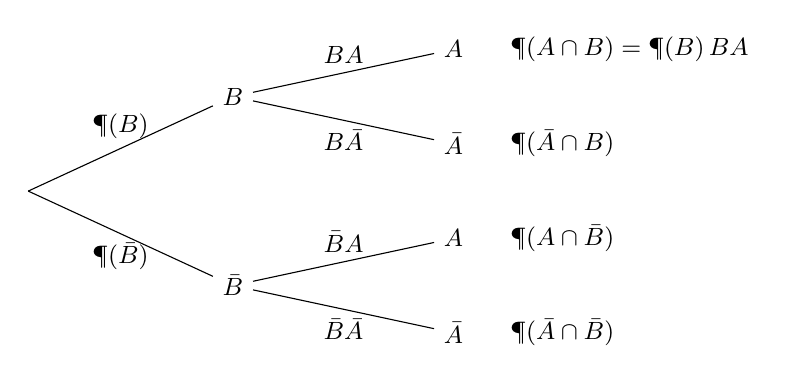
\begin{tikzpicture}[font=\small]
  \coordinate (root) at (0,0);
  \node (B)  at (2.6,1.2)  {$B$};
  \node (Bc) at (2.6,-1.2) {$\bar B$};
  \node (BA)  at (5.4,1.8)  {$A$};
  \node (BAc) at (5.4,0.6)  {$\bar A$};
  \node (BcA)  at (5.4,-0.6) {$A$};
  \node (BcAc) at (5.4,-1.8) {$\bar A$};
  \draw (root) -- (B)  node[midway, above] {$\P(B)$};
  \draw (root) -- (Bc) node[midway, below] {$\P(\bar B)$};
  \draw (B) -- (BA)   node[midway, above] {$\pcond{B}{A}$};
  \draw (B) -- (BAc)  node[midway, below] {$\pcond{B}{\bar A}$};
  \draw (Bc) -- (BcA)  node[midway, above] {$\pcond{\bar B}{A}$};
  \draw (Bc) -- (BcAc) node[midway, below] {$\pcond{\bar B}{\bar A}$};
  \node[anchor=west] at (6.0,1.8)  {$\P(A \cap B) = \P(B)\,\pcond{B}{A}$};
  \node[anchor=west] at (6.0,0.6)  {$\P(\bar A \cap B)$};
  \node[anchor=west] at (6.0,-0.6) {$\P(A \cap \bar B)$};
  \node[anchor=west] at (6.0,-1.8) {$\P(\bar A \cap \bar B)$};
\end{tikzpicture}

{\small A two-level tree: multiply along a path, add over the leaves.
For instance $\P(A)$ is the sum of the first and third leaf
probabilities.}
\end{omfigure}

\begin{theorem}[Bayes' formula]\label{thm:g12:condprob:bayes}
\index{Bayes' formula}
Let $B_1, \dots, B_n$ be a partition of $\Omega$ as above and $A$ an event
with $\P(A) > 0$. Then
\[
\pcond{A}{B_j} =
\frac{\P(B_j)\,\pcond{B_j}{A}}{\sum_{i=1}^{n} \P(B_i)\,\pcond{B_i}{A}} .
\]
\end{theorem}

\begin{proof}
$\pcond{A}{B_j} = \frac{\P(A \cap B_j)}{\P(A)}$; expand the numerator by
the multiplication rule and the denominator by total probability.
\end{proof}

\begin{example}[Screening test]\label{ex:g12:condprob:test}
A disease affects $1\%$ of a population. A test detects it with probability
$0.99$ (sensitivity) and gives a false positive with probability $0.05$.
Given a positive test, the probability of actually having the disease is
\[
\frac{0.01 \times 0.99}{0.01\times0.99 + 0.99\times0.05}
= \frac{0.0099}{0.0099 + 0.0495} = \frac{1}{6} \approx 0.17 .
\]
Despite the accurate test, five positives out of six are false --- because
the disease is rare. Confusing $\pcond{A}{B}$ with $\pcond{B}{A}$ is the
\emph{prosecutor's fallacy}.
\end{example}

\begin{omfigure}
\begin{tikzpicture}[font=\small]
  \coordinate (root) at (0,0);
  \node (D)  at (2.6,1.2)  {$D$};
  \node (Dc) at (2.6,-1.2) {$\bar D$};
  \node (DT)  at (5.2,1.8)  {$T$};
  \node (DTc) at (5.2,0.6)  {$\bar T$};
  \node (DcT)  at (5.2,-0.6) {$T$};
  \node (DcTc) at (5.2,-1.8) {$\bar T$};
  \draw (root) -- (D)  node[midway, above] {$0.01$};
  \draw (root) -- (Dc) node[midway, below] {$0.99$};
  \draw (D) -- (DT)   node[midway, above] {$0.99$};
  \draw (D) -- (DTc)  node[midway, below] {$0.01$};
  \draw (Dc) -- (DcT)  node[midway, above] {$0.05$};
  \draw (Dc) -- (DcTc) node[midway, below] {$0.95$};
  \node[omThm, anchor=west] at (5.8,1.8)  {$0.0099$ \ (true positives)};
  \node[anchor=west] at (5.8,0.6)  {$0.0001$};
  \node[omThm, anchor=west] at (5.8,-0.6) {$0.0495$ \ (false positives)};
  \node[anchor=west] at (5.8,-1.8) {$0.9405$};
\end{tikzpicture}

{\small The screening test as a tree ($D$: diseased, $T$: positive
test). The two positive leaves (red) have total weight $0.0594$, of
which the false positives contribute five sixths.}
\end{omfigure}

\section{Independence}

\begin{definition}[Independent events]\label{def:g12:condprob:indep}
Two events $A$ and $B$ are \emph{independent}\index{independence} if
\[
\P(A \cap B) = \P(A)\,\P(B) .
\]
When $\P(B) > 0$, this is equivalent to $\pcond{B}{A} = \P(A)$: knowing $B$
does not change the probability of $A$.
\end{definition}

\begin{proposition}\label{prop:g12:condprob:indepcompl}
If $A$ and $B$ are independent, so are $A$ and $\bar B$ (and $\bar A$ and
$\bar B$).
\end{proposition}

\begin{proof}
$\P(A \cap \bar B) = \P(A) - \P(A \cap B) = \P(A) - \P(A)\P(B)
= \P(A)\bigl(1 - \P(B)\bigr) = \P(A)\,\P(\bar B)$.
\end{proof}

\begin{remark}
Do not confuse \emph{independent} ($\P(A\cap B) = \P(A)\P(B)$) with
\emph{incompatible} ($A \cap B = \varnothing$). Two incompatible events of
nonzero probability are never independent: knowing one occurred guarantees
the other did not.
\end{remark}

\begin{definition}[Independent repetitions]\label{def:g12:condprob:repet}
When an experiment is repeated $n$ times so that the outcome of each trial
does not influence the others, the probability of a specified sequence of
outcomes is the product of the individual probabilities. This is the model
underlying the binomial distribution (\cref{ch:g12:randvar}).
\end{definition}

\section{Exercises}

\begin{exercise}[$\star$]\label{exo:g12:condprob:1}
A card is drawn from a standard 52-card deck. Compute the probability that
it is a king, given that it is a face card (jack, queen or king). Are the
events ``king'' and ``heart'' independent?
\end{exercise}

\begin{exercise}[$\star$]\label{exo:g12:condprob:2}
An urn contains 5 red and 3 blue balls. Two balls are drawn in succession
\emph{without} replacement.
\begin{enumerate}
  \item Draw the probability tree.
  \item Compute the probability that both are red, and the probability that
        the second is red.
\end{enumerate}
\end{exercise}

\begin{exercise}[$\star$]\label{exo:g12:condprob:3}
Two fair dice are rolled. Let $A$ = ``the sum is $7$'', $B$ = ``the first
die shows $3$'', $C$ = ``the sum is $6$''. Determine whether $A$ and $B$
are independent, then whether $B$ and $C$ are.
\end{exercise}

\begin{exercise}[$\star\star$]\label{exo:g12:condprob:4}
A factory has three machines producing respectively $50\%$, $30\%$ and
$20\%$ of total output, with defect rates $1\%$, $2\%$ and $4\%$.
\begin{enumerate}
  \item What proportion of the production is defective?
  \item A randomly chosen item is defective. What is the probability it
        came from the third machine?
\end{enumerate}
\end{exercise}

\begin{exercise}[$\star\star$]\label{exo:g12:condprob:5}
In \cref{ex:g12:condprob:test}, at what disease prevalence $p$ (instead of
$1\%$) would a positive test mean at least a $90\%$ chance of disease? Solve
the inequality and comment.
\end{exercise}

\begin{exercise}[$\star\star$]\label{exo:g12:condprob:6}
A biased coin lands heads with probability $p \in \intoo{0}{1}$. It is
tossed three times, tosses being independent.
\begin{enumerate}
  \item Compute the probability of the event $E$ = ``exactly two heads''.
  \item For which $p$ is $\P(E)$ maximal?
\end{enumerate}
\end{exercise}

\begin{exercise}[$\star\star\star$]\label{exo:g12:condprob:7}
\emph{(Monty Hall.)} A prize hides behind one of three doors. You pick a
door; the host, who knows where the prize is, opens one of the two
remaining doors, always revealing an empty one (choosing at random if both
are empty), and offers you to switch to the other closed door. Using
Bayes' formula, compute the probability of winning if you switch, and if
you do not.
\end{exercise}

\begin{exercise}[$\star\star\star$]\label{exo:g12:condprob:8}
An information channel transmits bits. Each bit is flipped by noise with
probability $\varepsilon = 0.1$, independently. To protect a bit, it is sent
three times and decoded by majority.
\begin{enumerate}
  \item Compute the probability that the decoded bit is wrong.
  \item The received word is $101$. What is the probability that the sent
        bit was $1$? (Assume $0$ and $1$ are sent with equal probability.)
\end{enumerate}
\end{exercise}
